\section{Symmetry and Goldstone's theorem}
\label{section:symmetry}

This section is based on \cite{Peskin:IntroQFT,weinberg_1995,weinberg_1996_vol2,smooth_manifolds}.

The symmetries of a theory are transformations of the physical state that leave the governing equations unchanged.
A lot of physics is contained in the symmetries of a theory, such as the presence of conserved quantities and the systems low energy behavior.
We distinguish between internal and external symmetries.
An external symmetry is an active coordinate transformation, such as rotations or translations.
They relate degrees of freedom at different space-time points, while internal symmetry transforms degrees of freedom at each space-time point independently of what happens at other points.
A further distinction is between local and global symmetry transformations.
Local transformations have one rule for how to transform degrees of freedom at each point, which is applied everywhere, while local transformations might themselves be functions of space-time.

In classical field theory, symmetries are encoded in how the Lagrangian changes due to a transformation of the fields.
We will consider continuous transformations, which are can in general be written as
\begin{equation}
    \varphi(x) \longrightarrow \varphi'(x) = f_t[\varphi](x), \quad t \in [0, 1].
\end{equation}
Here, $f_t[\varphi]$ is a functional in $\varphi$, and a smooth function of $t$, with the constraint that $f_0[\varphi] = \varphi$.
This allows us to look at ``infinitesimal'' transformations,
\begin{equation}
    \label{infinitesimal transformation}
    \varphi'(x) = f_\epsilon[\varphi] \sim \varphi(x) + \epsilon\diff{f[\varphi]}{t}\bigg |_{t=0}, \quad \epsilon \rightarrow 0.
\end{equation}
We will consider internal, global transformations which act as linearly on $\varphi$.
For $N$ fields, $\varphi_i$, this can be written
\begin{equation}
    \label{linear field transformation}
    \varphi_i'(x) = \varphi_i(x) + \epsilon \, i t_{ij} \varphi_j(x), \quad \epsilon \rightarrow 0.
\end{equation}
$t_{ij}$ is called the generator of the transformation.
A symmetry transformation the system is then a transformation in which the Lagrangian left is unchanged, or at most differ by a divergence-term.
That is, a transformation $\varphi \rightarrow \varphi'$ is a symmetry if 
\begin{equation}
    \Ell[\varphi'] = \Ell[\varphi] + \partial_\mu K^\mu[\varphi],
\end{equation}
where $K^\mu[\varphi]$ is a functional of $\varphi$.\footnote{Terms of the form $\partial_\mu K^\mu$ does not affect the physics, as variational principle $\delta S = 0$ do not vary the fields at infinity.}
This is a requirement for a symmetry in quantum field theory too.
However, as physical quantities in quantum field theory are given not just by the action of a single state but the path integral, the integration measure $\D \varphi_i$ has to be invariant as well.
If a classical symmetry fails due to the integration measure, it is called an anomaly.

To investigate the symmetry properties of a quantum theory, we explore what constraints a symmetry lies on the effective action.
To that end, assume 
\begin{equation}
    \D \varphi'(x) = \D \varphi(x), \quad
    S[\varphi'] = S[\varphi].
\end{equation}
In the generating functional, such a transformation corresponds to a change of integration variable.
Using the infinitesimal version of the transformation, we may write
\begin{align}
    \nonumber
    Z[J]
    = \int \D \varphi \, \exp{i S[\varphi] + i \int \dd^4 x J_i(x) \varphi_i(x)} 
    = \int \D \varphi' \, \exp{i S[\varphi'] + i \int \dd^4 x J_i(x) \varphi'_i(x)}
    \\
    = Z[J] -  \epsilon \int \dd^4 x J_i(x) \int \D \varphi \, e^{i S[\varphi]} [t_{ij} \varphi_j(x)],
\end{align}
Using \cref{effective equation of motion}, we can write this as
\begin{equation}
    \label{effective action symmetry requirement}
    \int \dd^4 x \, \fdiff{\Gamma[\varphi_J]}{\varphi_i(x)} \, t_{ij}\ex{\varphi_j(x)}_J = 0.
\end{equation}
This constraint will allow us to deduce the properties of a theory close to the ground state, only using information about the symmetries of the theory.


The arch typical example of an internal, global and continuous symmetry is the linear sigma model, which we will use as an example throughout this section.
The linear sigma model is made up of $N$ real scalar fields $\varphi_i$, which are governed by the Lagrangian
\begin{equation}
    \Ell[\varphi] 
    = \frac{1}{2} \partial_\mu \varphi_i(x) \partial^\mu \varphi_i(x) - \Ve(\varphi),
    \quad \Ve(\varphi) = - \frac{1}{2} \mu^2 \varphi_i(x)\varphi_i(x)
    + \frac{1}{4} \lambda [\varphi_i(x) \varphi_i(x)]^2.
\end{equation}
This system is invariant under the rotation of the $N$ fields into each other,
\begin{equation}
    \varphi_i \longrightarrow \varphi_i' = O_{ij} \varphi_j,
    \quad O^{-1} = O^{T}.
\end{equation}
The set of all such transformations form the Lie group $O(N)$.
Lie groups will be discussed in the next section.
For $N = 2$, and $\mu^2, \lambda > 0$ we get the famous Mexican hat potential, as illustrated in \autoref{fig:Mexican hat}.

\begin{figure}[ht]
    \centering
    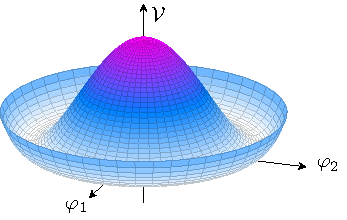
\includegraphics[width=0.6\textwidth]{figurer/mexican_hat.pdf}
    \caption{The Mexican hat potential is the classical potential $\Ve$ for the $N=2 $ linear sigma model.}
    \label{fig:Mexican hat}
\end{figure}

\subsection*{Lie groups}
(HA I APPENDIX?)

Lie groups are a natural structure to capture the symmetries of a theory.
A Lie group is a smooth manifold, i.e. a space that is locally diffeomorphic to $\R^N$.
This means that we can locally parametrize the space by $N$ real numbers $\eta_\alpha$, using smooth invertible functions.
A Lie group is also equipped with group structure.
A group is a set, $G$, together with a map
\begin{align}
    (\cdot, \cdot):  G \times G &\longmapsto G ,\\
    (g_1, g_2) &\longmapsto g_3,
\end{align} 
called group multiplication. This map obeys the group axioms, which are the existence of an identity element $\one$, associativity and the existence of an inverse element $g^{-1}$ for all $g\in G$.
These can be written as
\begin{table}[!h]
    \centering
    \begin{tabular}{l l}
        $\forall g \in G, $&$ (g, \one) = g, $\\
        $\forall g_1, g_2, g_3 \in G, $ & $ (g_1, (g_2, g_3)) = ((g_1, g_2), g_3), $\\
        $\forall g \in G,\, \exists g^{-1} \in G,\, \text{s.t.}, $ & $ (g, g^{-1}) = \one.$
    \end{tabular}
\end{table}

In addition, we require that both the multiplication map and the inverse map, $g \mapsto g^{-1}$ are smooth.
We describe the set of continuous symmetry transformations, 
\begin{equation}
    G = \setbuilder{g}{g \varphi = \varphi', \, S[\varphi'] = S[\varphi], \D \varphi' = \D \varphi },
\end{equation}
as a Lie group, where the group multiplication is composition, i.e. performing transformations in succession.
This map is closed, as two symmetry transformations are another symmetry transformation.
The identity map is a symmetry transformation, and composition is associative.
This means that invertible symmetry transformations form a group.

We will focus on connected Lie groups, in which we all elements $g \in G$ is in the same connected piece as the identity map $\one \varphi = \varphi$.
This means that for each $g\in G$, one can find a continuous path $\gamma(t)$ in the manifold, such that $\gamma(0) = \one$ and $\gamma(1) = g$.
Given such a path, we can study transformations close to the identity.
As the Lie group is a smooth manifold, we can write\footnote{The factor $i$ is a physics convention, and differs from how mathematicians define generators of a lie group.}
\begin{equation}
    \gamma(\epsilon) = \one + i \epsilon V + \Oh{\epsilon}
\end{equation}
$V$ is a generator, is defined as
\begin{equation}
    iV = \diff{\gamma}{t}\Big|_{t=0}.
\end{equation}
We can define a path $\gamma$ by its path through parameter space, $\gamma(t) = g(\eta(t))$, which means that we can write the generator as
\begin{equation}
    V = \diff{\gamma}{t}\Big|_{t=0} = \diff{\eta_a}{t}\Big|_{t=0} \diffp{g}{\eta_a}\Big|_{\eta=0}
    = \diffp{g}{\eta_a}\Big|_{\eta=0} T_\alpha, \quad 
    T_\alpha = \diffp{g}{\eta_\alpha}.
\end{equation}
We see that the generators form a vector space, with the basis $T_\alpha$, induced by the coordinates $\eta_a$.
This vector space is called the tangent space of the identity element, $T_\one G$.
Infinitesimal transformations can therefore be written as
\begin{equation}
    \gamma(\epsilon) = \one + i \epsilon v_\alpha T_\alpha, \quad \epsilon \rightarrow 0.
\end{equation}
The tangent space, together with the additional operation
\begin{align}
    [T_\alpha, T_\beta] = iC_{\alpha\beta}^\gamma T_\gamma,
\end{align}
called the Lie bracket, forms a Lie algebra denoted $\mathfrak{g}$.
For matrix groups, which are what we deal with in this text, the Lie bracket is the commutator.
$C_{\alpha \beta}^\gamma$ are called structure constants.
They obey the Jacobi identity,
\begin{equation}
    \label{jacobi identity}
    C_{\alpha \beta}^\gamma + C_{\beta\gamma}^\alpha +  C_{\gamma\alpha}^\beta = 0,
\end{equation}
which mean that they are totally antisymmetric.
A subset of the original Lie group, $H \subset G$, which is closed under the group action is called a subgroup.
$H$ then has its own Lie algebra $\mathfrak{h}$, with a set of $m = \dim H$ generators, $x_i$, which is a subset of the original generators $T_\alpha$
We denote the remaining set of generators $t_a$, such that $x_i$ and $t_a$ together span $\mathfrak{g}$.

Of special importance are one parameter subgroups.
If a curve $\gamma(t)$ through $G$ obey
\begin{equation}
    \gamma(t)\gamma(s) = \gamma(t + s), \quad \gamma(0) = \one,
\end{equation}
then all the points on this curve from a one parameter subgroup of $G$.
This path is associated with a generator, 
\begin{equation}
    \diff{\gamma}{t} \Big|_{t=0} = i \eta_\alpha T_\alpha.
\end{equation}
This allows us to define the exponential map,
\begin{equation}
    \exp{i \eta_\alpha T_\alpha} := \gamma(1).
\end{equation}
For connected and compact Lie groups, all elements of the Lie group $g \in G$ can be written as an exponential of elements in the corresponding Lie algebra $\eta_\alpha T_\alpha \in \mathfrak g$.
For matrix groups, the exponential equals the familiar series expansion
\begin{equation}
    \exp{X} = \sum_n \frac{1}{n!} X^n.
\end{equation}

A subgroup $H \in G$ has its own Lie algebra $\mathfrak{h}$, with a set of $m = \dim H$ generators, $x_i$, which is a subset of the original generators $T_\alpha$.
We denote the remaining set of generators $t_a$, such that $x_i$ and $t_a$ together span $\mathfrak{g}$.
The commutators of $x_i$ must be closed, which means that we can write
\begin{align}
    [x_i, x_j] &= i C_{i j}^{k} x_k,\\
    [x_i, t_a] &= i C_{i a}^b t_b, \\
    [t_a, t_b] &= i C_{ab}^k x_k + i C_{ab}^c t_c,
\end{align}
where $ijk$ runs over the generators of $\mathfrak h$, and $abc$ runs over the rest.
The second formula can be derived using the Jacobi identity \cref{jacobi identity}, which implies that $C_{ia}^k = -C_{ik}^a = 0$.
This is called a Cartan decomposition.

\subsection*{Nöther's theorem}

One of the most profound consequences of symmetry in physics is the appearance of conserved quantities.
Assume we have a set of fields $\varphi_i$. Nöther's theorem tells us that if the Lagrangian $\Ell[\varphi_i]$ has a ontinuous symmetry, then there is a corresponding conserved current~\cite{Peskin:IntroQFT,Carroll:spacetime}.
Consider an infinitesimal transformation,
\begin{equation*}
    \varphi_i(x) \longrightarrow \varphi_i'(x)
    \sim \varphi_i(x) + \delta \varphi_i(x),.
\end{equation*}
Applying this transformation to the Lagrangian will in general change its form,
\begin{equation*}
    \Ell[\varphi_i] \rightarrow \Ell[\varphi_i']
    \sim \Ell[\varphi_i] + \delta \Ell.
\end{equation*}
If the change in the Lagrangian can be written as a total derivative, i.e.
\begin{equation*}
    \delta \Ell = \partial_\mu K^\mu(x).
\end{equation*}
Nöther's theorem states that the current
\begin{equation}
    j^\mu = \pdv{\Ell}{(\partial_\mu \varphi_i)} \delta \varphi_i(x) - K^\mu
\end{equation}
obeys the conservation law
\begin{equation}
    \partial_\mu j^\mu = 0.
\end{equation}
The flux of current through some space-like surface $V$, i.e. a surface with a time-like normal vector, defines a conserved charge. This surface is most commonly a surface of constant time in some reference frame. The conserved charge is then
\begin{equation*}
    Q = \int_V \dd^3 x \, j^0.
\end{equation*} 
Using the divergence theorem again, and assuming the current falls of quickly enough towards infinity, we can show that the total charge is conserved,
\begin{equation*}
    \pdv{t} Q = - \int_V \dd^3 x \, \nabla \cdot \vec j = - \int_{\partial V} \dd^2 x\, n_\mu j^\mu = 0.
\end{equation*}
Here, $n^\mu$ is the time-like normal vector of the surface of $V$, $\partial V$.


\subsection*{Goldstone's theorem}

The fact that a theory is left invariant under some symmetry transformation does not imply that the ground state is invariant under this transformation.
The $N = 2$ linear sigma model illustrates this.
If we assume the ground state $\varphi_{0}$ is translationally invariant, then it is given by minimizing the effective potential, of which the classical potential, $\Ve$, is the leading order approximation.
This potential is illustrated in \autoref{fig:Mexican hat}.
The ground state is therefore given by any of the values along the brim of the potential.
If we, without loss of generality, choose $\varphi_0 = (0, v)$ as the ground state, then any symmetry transformation will change this state.
We say that the symmetry has been \emph{spontaneously broken}.

To explore this in a general context, assume a theory of $\varphi_i$ real scalar fields are invariant under the actions of some Lie group, $G$.
A symmetry $g \in G$ is broken if the vacuum expectation value of the original fields and the transformed fields differ.
That is, if
\begin{equation}
    \ex{\varphi}_0 \neq \ex{\varphi'}_0 = \ex{g \varphi}_0
\end{equation}
We can now exploit what we learned about Lie groups to write
\begin{equation}
    \ex{\varphi'}_0 = \ex{\varphi}_0 + i \epsilon \eta_\alpha T_\alpha \ex{\varphi}_0.
\end{equation}
Let $t_a$ be the set of generators corresponding to broken symmetries, i.e.
\begin{equation}
    t_\alpha \ex{\varphi}_0 \neq 0.
\end{equation}
These are called the \emph{broken generators}.
The remaining set of generators $x_i$, which obey
\begin{equation}
    x_i \ex{\varphi}_0 = 0,
\end{equation}
are called unbroken, and generate a subgroup $H \subset G$ as the set of symmetry transformations of the vacuum is a group.

In \cref{effective equation of motion} we found that the effective action obey
\begin{equation}
    \int \dd^4 x \fdiff{\Gamma[\varphi_J]}{\varphi_i} t_{ij} \ex{\varphi_j}_0 = 0.
\end{equation}
We now differentiate this expression with respect to $\varphi_k(y)$ and evaluate it in the vacuum, which gives
\begin{equation}
    \int \dd^4 x \, \fdiff{\Gamma[\varphi_0]}{\varphi_k(y), \varphi_i(x)}
    t_{ij} \ex{\varphi_j}_0 = 0.
\end{equation}
With the assumption that the ground state is constant, we get 
\begin{equation}
    \diffp{\Veff}{\varphi_k, \varphi_i} \, t_{i j} \ex{\varphi_j}_0 = 0.
\end{equation}
This is trival for unbroken symmetries, as $t_{ij}\ex{\varphi_j}_0 = 0$ by definition.
However, in the case of a broken symmetry, the second derivative of the effective potential has an eigenvector $t^\alpha_{ij} \ex{\varphi_j}$ with a zero eigenvalue for each broken generator.
In \autoref{Effective action inverse propagator}, we found that the second derivative of the effective action is the inverse propagator,
\begin{equation}
    D^{-1}_{ij}(x,y) 
    = -i \fdiff{\Gamma[\varphi_0]}{\varphi_i(y), \varphi_j(x)}
    = \int \frac{\dd^4 p}{(2 \pi)^4} e^{-ip(x - y)} \, \tilde D^{-1}_{ij}(p).
\end{equation}
Using this, we can write
\begin{equation}
    \tilde D^{-1}_{i j}(p=0) \, t^\alpha_{j k} \ex{\varphi_k}_0 
    = 0.
\end{equation}
Zeros of the inverse propagator corresponds to the physical mass of particles.
In Lorentz-invariant systems, each zero-mass vector corresponds to a masses particles, called a Goldstone boson.\footnote{ The particles are bosons due to the bosonic nature of the transformations, $t$. If the generators are Grassmann numbers, the resulting particle, called goldstinos, are fermions.}
This means there are $n_G = \dim G -\dim H$ zero mass modes.
In general, counting of massless modes is complicated, and depends on the dispersion relation of the particles at low momenta.
Systems with Goldstone bosons with quadratic dispersion relation, that is $E = |\vv p|^2$ when $\vv p \rightarrow 0$, often exhibit a lower number of massless modes.
An example is ferromagnets, where the $\mathrm{SU}(2)$ rotational symmetry is broken down to $\mathrm{U}(1)$ when they align along one axis. 
This corresponds to two broken generators, yet the system exhibits only one massless mode~\cite{brauner_spont_sym}.

\begin{figure}[ht]
    \centering
    \begin{subfigure}{0.54\textwidth}
        \centering\captionsetup{width=.9\linewidth}
        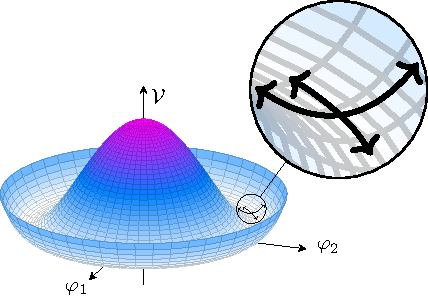
\includegraphics[]{figurer/mexican_hat_zoom.pdf}
        \caption{Excitations along the brim does not cost any energy, as the potential is flat, unlike excitations in the radial direction.}
        \label{fig:Mexican hat zoom}
    \end{subfigure}
    \begin{subfigure}{0.45\textwidth}
        \centering\captionsetup{width=.9\linewidth}
        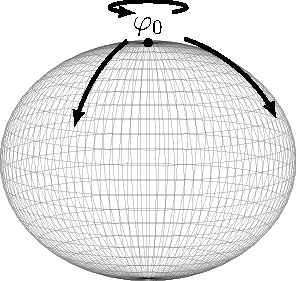
\includegraphics[]{figurer/sigma_ground_state.pdf}
        \caption{Excitations for the $N=3$ sigma model. Two of the symmetries are broken, while rotations around the groundstate leaves the system unchanged.}
        \label{fig:ground state manifold}
    \end{subfigure}
\end{figure}

The linear sigma model gives an intuition for the Goldstone mode.
In the case of $N = 2$, the symmetry of the Lagrangian are rotations in the plane.
As the ground state is a point along the ``brim'' of the hat, this rotational symmetry is broken.
Any excitations in the rotational direction, however, does not cost any energy, which is indicative of a massless mode.
This is illustrated in \autoref{fig:Mexican hat zoom}.
In this example, the original symmetry group is one dimensional, so there are no unbroken symmetries.
If we instead consider the $N=3$ linear sigma model, which has a three-dimensional symmetry group, rotations of the sphere, we see that the ground state is left invariant under subgroup of the original symmetry transformations.
The ground state manifold of this system, the set of all states that minimizes the effective potential, is then a sphere.
When the system chooses one single ground state, this symmetry is broken, but only for two of the generators. 
The generator for rotations around the ground state leaves the that point unchanged, and is thus an unbroken symmetry.
Any excitations in the direction of the broken symmetries does not cost energy, as it is in the ground state manifold.
The unbroken symmetry, on the other hand, does not correspond to an excitation.
This is illustrated in \autoref{fig:ground state manifold}.

